\section{How we got here}
\label{sec:story}

The starting point was a small network that should have been able to solve its
task. The QDO study used an eight-dimensional input and a teacher built from four
orthogonal features, each rectified separately. A four-unit student already had
enough architectural capacity to implement that teacher. Nevertheless, some
training runs converged to representations that merged distinctions the answer
still depended on. The failure was visible inside the computation: different
inputs could reach the same complete intermediate state while requiring different
outputs \cite{qdo,projection}.

One especially useful picture was a pair of teacher features \(A\) and \(B\)
whose output coefficients have the same sign. Their input-dependent
preactivations need not share a sign. A failed
representation could keep their common direction, \(A+B\), while weakening their
contrast, \(A-B\). In one diagnosed cohort, geometric retention was about
\(99.6\%\) for the common direction and \(27.7\%\) for the contrast. These are
geometric measurements from that cohort, not percentages of information or of
all model error. The distinction mattered because
\[
  \ReLU(A)+\ReLU(B)\ne\ReLU(A+B)
\]
in general. A positive contribution can disappear when it is first combined with
a negative contribution and only then rectified. The project also certified a
second failure: preactivations that remained different after the linear map
became identical after ReLU \cite{qdo,projection}.

QDO approached the problem through optimization. Its historical anchors lived in
parameter-derived coordinates, and its repulsive update tried to move training
away from configurations already visited. The invariant version removed a
per-neuron scaling ambiguity before measuring those distances. That is a different
intervention from saving an activation contrast. The manuscript reports a
bounded synthetic continuation study; it does not establish a general optimizer
or a guarantee of information preservation. In the present research discussion,
QDO was judged unsuccessful as the direction to pursue and was set aside. This
proposal carries forward the diagnostic lessons, rather than reopening that
optimizer \cite{qdo,discussion}.

The next intuition was deliberately visual. Imagine arbitrary patterns on a
\(9\times9\) grid. Rotate them, place them over one another, and ask what the
result still tells us about the original views. Ordinary addition can make
different patterns indistinguishable. The suggestion was to make overlapping
contributions darker, so that overlap itself leaves a record. The idea quickly
acquired two further requirements: a pile may contain more than two layers, and
the order of the layers matters. Upper layers should receive different, heavier
weights, but those weights must not become another way to erase a lower layer's
contribution.

An early mathematical detour treated the requirement of no lost information as
exact recovery of every original input bit. That led to positional integer
encodings, capacity bounds, and invertible mixtures of known rotations. Those
calculations were useful boundaries: a single ordinary weighted sum cannot
encode arbitrary independent real-valued layers, while known rotations of one
source are a different problem. They also exposed how floating-point rounding
can defeat an algebraic inverse. But complete serialization was a stronger
requirement than the developing proposal needed. These results remain in an
appendix so that the change of objective is explicit.

The decisive clarification brought back the earlier Hodge atlas work. In the
project's description, local charts already have overlaps, transition maps,
consistency conditions, and a reconstruction or gluing step. The question became:
what must survive between two neural slices so that these local descriptions
still determine the target when glued together? A contrast such as \(A-B\) is
one candidate. The required record can be smaller than a complete copy of the
input if every ambiguity it leaves is irrelevant to the required computation
\cite{discussion}.

Recurrent Dragon supplied a related discipline in the research discussion:
respect causal order, distinguish a useful predictive state from a record of the
entire history, and do not infer a preservation guarantee from predictive success.
The present design also keeps actual transition data and nonlinear interactions
available; it does not substitute scalar coalition attributions for them.
Those are design constraints from prior-work discussion, not claims that this
proposal has inherited a previously verified implementation \cite{discussion}.

CReLU then provided a concrete comparison. It retains both positive and negative
parts of a measured response \cite{crelu}. The proposed mechanism asks whether only selected
contrasts or correction quantities need this protection, with atlas reconstruction
aligning them across slices. The proposal is therefore to \emph{capture
target-relevant distinctions before they disappear, preserve their layer and
chart identities, and glue the retained records into a representation whose
remaining ambiguities cannot change the target}.

\begin{keybox}
\textbf{Central claim to establish.}
For a declared target or target family \(T\), the complete retained representation
\(E\) must satisfy
\[
  E(x)=E(x')\quad\Longrightarrow\quad T(x)=T(x').
\]
Overlap compatibility organizes reconstruction. This implication supplies the
information-preservation requirement.
\end{keybox}

\section{Proposal, scope, and evidence}
\label{sec:overview}

The proposed forward computation has an ordinary path and a selective record
path. At a boundary where a projection, merge, activation, or later aggregation
could discard a target-relevant distinction, a small record is emitted from the
information that still exists before that operation. The record carries a layer
index and, when needed, a chart or branch identity. Existing atlas maps relate
records on overlaps. A reconstruction step combines the records with the
ordinary state, and a readout consumes the resulting representation.

\begin{figure}[htbp]
 \centering
 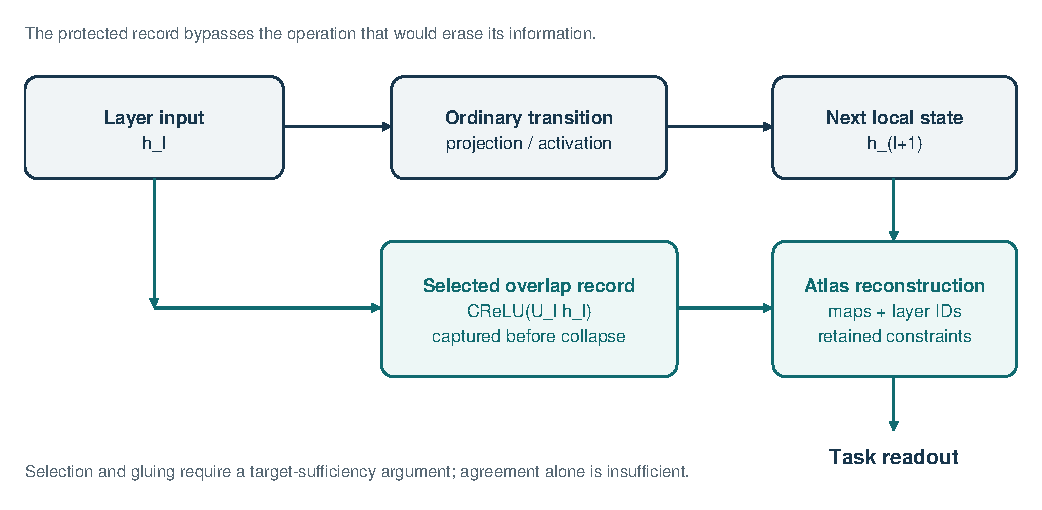
\includegraphics[width=\linewidth]{figures/architecture.pdf}
 \caption{Proposed information path. The record is measured before the
 destructive transition. Its selected coordinates and the reconstruction both
 require a target-sufficiency argument. The diagram does not assume that every
 neural layer is an invertible chart.}
\end{figure}

The main objective is preservation of a declared computation or task family.
Full input reconstruction is a useful reference case, obtained by setting
\(T(x)=x\), but it is not imposed by default. Exact order recovery is a separate
requirement whenever order or source identity must survive independently of the
target value. Such metadata remains explicit.

\begin{center}
\small
\begin{tabularx}{\linewidth}{@{}p{0.27\linewidth}X@{}}
\toprule
Status & What is supported in this proposal\\
\midrule
Proved algebra & Target-factorization criterion; exact ReLU cancellation
correction; finite merge identities; linear target observability; minimal
linear side records; weighted reconstruction and stability bounds.\\
Checked examples & Deterministic finite-domain checks and explicit negative
controls, reproduced by the supplied verification script.\\
Proposed design & Learned selective records, chart transport, record budgets,
and an end-to-end neural readout. These have not been trained here.\\
Not established & A general learning guarantee, lower total compute,
superiority to CReLU or ordinary added capacity, or preservation of every
possible future task.\\
\bottomrule
\end{tabularx}
\end{center}

\paragraph{Provenance.}
QDO and projection-audit statements come from the inspected project manuscript
and report \cite{qdo,projection}. The Hodge atlas mechanism and Recurrent Dragon
lessons are used as described in the research discussion \cite{discussion};
their implementations were not independently re-audited for this proposal.
Public literature supplies comparison points, not evidence that the proposed
neural system already works. The derivations state their assumptions and make
no claim that the elementary identities themselves are new.

\clearpage
\tableofcontents
\newpage

\section{The exact preservation criterion}
\label{sec:sufficiency}

Let \(\mathcal X\) be the allowed source domain and let
\[
 T:\mathcal X\to\mathcal Y
\]
be the target, task-feature vector, or specified collection of downstream
quantities. Let \(E:\mathcal X\to\mathcal E\) include \emph{everything} retained:
ordinary hidden state, side records, layer indices, branch labels, anchors, and
any input-dependent transition metadata.

\begin{theorem}[Target sufficiency]
\label{thm:fibers}
There exists a decoder \(D:E(\mathcal X)\to\mathcal Y\) satisfying
\begin{equation}
 T=D\circ E
 \label{eq:factorization}
\end{equation}
if and only if
\begin{equation}
 E(x)=E(x')\ \Longrightarrow\ T(x)=T(x')
 \qquad\text{for all }x,x'\in\mathcal X.
 \label{eq:fibers}
\end{equation}
\end{theorem}
\begin{proof}
If \(T=D\circ E\), equal encodings have equal decoded targets. Conversely,
for each \(e\in E(\mathcal X)\), choose any \(x\) with \(E(x)=e\) and define
\(D(e)=T(x)\). Condition \eqref{eq:fibers} makes this definition independent
of the chosen preimage.
\end{proof}

The encoder may identify distinct source states, but only when they have the
same required target. Every fiber \(E^{-1}(e)\) must lie inside a target
fiber. Decoder existence is a structural statement; it does not imply that
decoding is cheap, stable, continuous, or learnable from finite data.

For an existing retained state \(h\), if a fiber \(h^{-1}(z)\) contains \(N_z\)
distinct required target values, an added record must have at least \(N_z\)
distinguishable states on that fiber. For a finite digital alphabet, this
requires at least \(\lceil\log_2N_z\rceil\) fixed-width record bits on that
fiber. The needed capacity depends on missing target distinctions, rather
than automatically on every missing input distinction.

\subsection{Task families and unknown future use}

For a family \(\mathcal F\) of future readouts, require
\[
 E(x)=E(x')\Longrightarrow
 f(x)=f(x')\quad\text{for every }f\in\mathcal F.
\]
For a finite family, take \(T=(f_1,\ldots,f_q)\). If every possible source
distinction matters to some allowed future task, the requirement becomes full
injectivity. A selective guarantee therefore needs a declared task family.
Keeping a currently known scalar answer can be much easier than keeping the
computation reusable for other answers.

For a streaming state with unknown future inputs, two histories may be merged
only if every allowed future continuation produces the same required outputs.
Agreement on the current prefix's answer alone does not establish this.

\subsection{The distributional counterpart}

For a deterministic square-integrable scalar target \(Y=T(X)\), the best
squared-error decoder from \(E(X)\) is the conditional mean. Its risk is
\begin{equation}
 R_E=\E\!\left[\Var(Y\mid E(X))\right].
 \label{eq:bayesrisk}
\end{equation}
For any decoder \(\widehat Y=g(E(X))\),
\begin{equation}
 \E[(Y-\widehat Y)^2]
 =R_E+
 \E\!\left[
 \bigl(\E[Y\mid E(X)]-g(E(X))\bigr)^2
 \right].
 \label{eq:bayesdecomp}
\end{equation}
Expand the squared error around the conditional mean. The cross term has
conditional expectation zero, proving the identity.

Thus \(R_E=0\) gives exact target determination almost surely under the source
distribution. It is not a guarantee on inputs outside that support or on
measure-zero exceptions. A finite set of successful reconstructions is weaker.
For intrinsically noisy labels, preserving the complete predictive law
requires preserving the conditional target distribution. If the declared
objective is squared error alone, preserving the conditional mean suffices
to attain the full-information Bayes risk. Zero conditional variance would
instead incorrectly demand removal of irreducible label noise.

\subsection{Sequential preservation}

Let \(s_\ell=(h_\ell,m_\ell)\) be the complete carried state, including earlier
records. A boundary update may have the form
\[
 s_{\ell+1}=G_\ell(s_\ell)
 =\bigl(F_\ell(h_\ell),m_\ell,r_\ell(s_\ell)\bigr).
\]
\begin{proposition}[Composition]
If \(T_0=T\) and, on reachable states, each stage admits \(T_{\ell+1}\) with
\[
 T_\ell=T_{\ell+1}\circ G_\ell,
\]
then
\[
 T=T_L\circ G_{L-1}\circ\cdots\circ G_0.
\]
\end{proposition}
\begin{proof}
Substitute the stage factorizations successively.
\end{proof}

If earlier records are compressed or removed, that operation is another stage
to which the same condition applies. A local record can be sufficient together
with other records without being sufficient by itself. The complete carried
state, rather than an isolated side channel, is the object to audit.
